\documentclass[12pt,a4paper]{article}

\usepackage[T1]{fontenc}
%\usepackage[polish]{babel}
\usepackage{polski}
\usepackage[utf8]{inputenc}
\usepackage{caption}
\usepackage[newfloat]{minted}
\usepackage{lmodern}
% pakiet dodaje wcięcie do pierwszego paragrafu po
% tytule. Domyślnie pierwszy nie ma wcięcia.
\usepackage{indentfirst}
\usepackage{graphicx}
\usepackage[top=2.5cm, bottom=2.5cm, left=2.5cm, right=2.5cm]{geometry}
\usepackage{setspace}
\usepackage{hyperref}
\usepackage[parfill]{parskip}
\hypersetup{
	colorlinks,
	citecolor=black,
	filecolor=black,
	linkcolor=black,
	urlcolor=black	
}
%\usepackage{times}
\usepackage{tgtermes}
\usepackage{array}
\usepackage{multirow}
\usepackage{wrapfig}
% \usepackage{listings}
\usepackage{chngcntr}
\usepackage{longtable}
\setcounter{secnumdepth}{3}
\graphicspath{{images/}}

\renewcommand*{\figurename}{Rys.}
\renewcommand*{\tablename}{Tab.}
% \renewcommand*{\listingname}{Kod.}
\renewcommand{\thelisting}{\arabic{section}.\arabic{listing}}
\renewcommand{\thetable}{\arabic{section}.\arabic{table}}
\renewcommand{\thefigure}{\arabic{section}.\arabic{figure}}

\counterwithin{figure}{section}
\counterwithin{table}{section}

\begin{document}
	\nocite{*}
	\pagenumbering{gobble}
	% strona tytułowa
	\begin{titlepage}
	% logo WI i ZUT
	\begin{figure}[!htb]
		\begin{minipage}{0.48\textwidth}
			\raggedright
			
\includegraphics[width=0.8\linewidth]{ZUT_2.jpg}
		\end{minipage}\hfill
		\begin{minipage}{0.48\textwidth}
			\raggedleft
			
\includegraphics[width=0.8\linewidth]{WI_2.jpg}
		\end{minipage}
	\end{figure}
	\vspace{2cm}
	\begin{center}
		\textbf{Piotr Zieliński}\\
		Nr albumu: 29979
	\end{center}
	\begin{center}
		Kierunek studiów: Informatyka\\
		Forma studiów: studia stacjonarne
	\end{center}
	\vspace{1.5cm}
	\begin{center}
		\textbf{\LARGE System płatności w strefie płatnego parkowania z wykorzystaniem urządzeń mobilnych oraz kodów QR}
	\end{center}
	\begin{center}
		{\large A payment system in a paid parking zone with mobile devices and QR codes}
	\end{center}
	\vspace*{\stretch{6}}
	\begin{center}
		Praca dyplomowa inżynierska\\
		napisana pod kierunkiem:\\
		\textbf{dr inż. Edwarda Półrolniczaka\\
			Katedra Systemów Multimedialnych}
	\end{center}
	\vspace{.5cm}
	%\noindent
	Data wydania tematu pracy:\\
	Data złożenia pracy:
	
	\begin{center}
		Szczecin, 2016
	\end{center}

\end{titlepage}
	
	% pusta strona
	%\mbox{}
	%\thispagestyle{empty}
	%\newpage
	
	\begin{onehalfspacing}
		
		% oświadczenie
		\topskip0pt

\vspace*{\fill}

\begin{center}
	{\large \textbf{OŚWIADCZENIE\\AUTORA PRACY DYPLOMOWEJ}}
\end{center}

\vspace{1cm}

Oświadczam, że praca dyplomowa inżynierska pn.

\begin{center}
	System płatności w strefie płatnego parkowania z wykorzystaniem urządzeń mobilnych oraz kodów QR
\end{center}

napisana pod kierunkiem:

\begin{center}
	dra inż. Edwarda Półrolniczaka
\end{center}

jest w całości moim samodzielnym autorskim opracowaniem sporządzonym przy wykorzystaniu wykazanej w pracy literatury przedmiotu i materiałów źródłowych. 

Złożona w dziekanacie

\begin{center}
	Wydziału Informatyki
\end{center}

treść  mojej pracy dyplomowej w formie elektronicznej jest zgodna z treścią w formie pisemnej i graficznej.

Oświadczam ponadto, że złożona w dziekanacie praca dyplomowa ani jej fragmenty nie były wcześniej przedmiotem procedur procesu dyplomowania związanych z uzyskaniem tytułu zawodowego w uczelniach wyższych.

\vspace{2cm}

\begin{flushright}
	\begin{tabular}{ c }
		{\footnotesize ....................................}\\[-.8em]
		{\footnotesize podpis dyplomanta}
	\end{tabular}
\end{flushright}

\vspace{1cm}

{\footnotesize Szczecin, dn. ....................................}

\vspace*{\fill}
		\newpage
		
		%abstract
		\topskip0pt

\vspace*{\fill}

\begin{center}
	{\large \textbf{ABSTRACT}}
\end{center}

\vspace{1cm}

The aim of this thesis was to create a payment system for a paid parking zone, which allows to buy and control a parking ticket by a mobile applications. QR codes were used for vehicle identification in the system.

The main tasks associated with this thesis was to implement two mobile applications, separately for a driver and a parking officer. First of them can create a new account, add vehicles and buy tickets. A parking officer from its application can control tickets validity, by scanning badges which contains QR codes.

The first chapter describes the online payments. There are informations about their history, payments methods and gateways. Next chapter is about technologies, that were used in implementation. There is described the Django framework, the Android mobile system and QR codes. The third chapter mostly contains the system specification with UML diagrams, functional and non-functional requirements. The last part is about results of the working system, with description and screenshots from web and mobile applications.

\vspace*{\fill}
		\newpage
		
		% spis treści
		\pagenumbering{arabic}
		\setcounter{page}{3}
		\tableofcontents
		\newpage
		
		% wstęp
		\section*{Wstęp}
\addcontentsline{toc}{section}{Wstęp}

Internet oraz płatności elektroniczne przez lata wzajemnie kształtowały swój rozwój. 
		\newpage
		
		\section{Płatności elektroniczne}

\subsection{Wprowadzenie}

% przejście od e-commerce do płatności, gdzie się z nimi spotykamy
E-commerce często utożsamia się tylko z dokonywaniem zakupów przez internet. Tymczasem występował już wcześniej pod wieloma postaciami i dotyczy m.in. telefonu, faksu, czy telewizji. Odnosi się ogólnie do stosowania urządzeń elektronicznych w zakupie oraz sprzedaży. Jednak to właśnie internet jest dominującą obecnie formą e-handlu, będąc medium informacyjnym łączącym niejako wszystkie poprzednio używane. Jego nieograniczone wręcz możliwości przyciągają nowych użytkowników, którzy z czasem nabierają zaufania i stają się także kupującymi. W ten sposób dynamiczny rozwój sieci napędza także handel elektroniczny. Przedsiębiorcy chcąc zachować kontakt z klientami muszą zaznaczyć swoją obecność tam, gdzie koncentruje się większa część aktywności ludzkiej. Owocuje to powstawaniem nowych sklepów internetowych.

% definicja e-płatności
Płatności elektroniczne to bezgotówkowa formą zawierania transakcji. Są to wszelkiego rodzaju operacje finansowe zawierane kanałami elektronicznymi. Możemy zaliczyć do nich m.in. karty płatnicze, czy polecenia przelewu. Bardzo zyskujące ostatnio na popularności są płatności internetowe, dokonywane za pośrednictwem sieci internetowej. Mogą być realizowane różnymi kanałami, a należą do nich chociażby płatności kartą płatniczą, przelewy bankowe czy e-portmonetki. Transakcje takie zawierane są na odległość, za pośrednictwem urządzeń (instrumentów) elektronicznych - komputerów, tabletów lub smartfonów. Napotkać można się na nie w serwisach aukcyjnych, czy sklepach internetowych gdzie występują jako jedna z form zrealizowania opłaty za produkt lub usługę. 

Handel internetowy nie mógł by istnieć bez płatności internetowych. To właśnie wspólny rozwój e-handlu z internetem umożliwił powstanie nowej metody zawierania transakcji. Dzięki temu są one dobrze przystosowane do wymagań stawianych w rozwiązaniach z dziedziny e-commerce. Oferują one szybkość oraz wygodę w zawieraniu transakcji. Dzięki coraz większej konkurencji pomiędzy dostawcami usług płatniczych - także korzystniejsze prowizję. Ich zastosowanie rośnie, wraz z rosnącą liczbą usług oferowanych w internecie. Szczególnie zaznaczyły swoja obecność w aplikacjach mobilnych. Opłaty mogą być związane z uzyskaniem dostępu do takiego programu, bądź dodatkowej treści.

% gdzie teraz sę e-płatności
Po kilkunastu latach płatności elektroniczne dalej są w fazie dynamicznego rozwoju. Dzięki rozwojowi technologii znajdują się dla nich cały czas nowe zastosowania. 

\subsection{Historia i etapy rozwoju}

% TODO Tu od początku o płatnościach - pieniądz elektroniczny, internet, bankowość. Bez opisu jak działają, tylko jak do nich doszło.

Powstanie płatności elektronicznych związane jest przede wszystkim z bankowością elektroniczną.

%TODO obszerny opis jak doszło do powstania płatności

\paragraph{Pierwsza generacja}

\paragraph{Druga generacja}

\subsection{Charakterystyka}

% TODO Wszelakie podziały - mikropłatności, bcb, rodzaje płatności. Także opis jak działają, co to jest - dokładniejsze od wprowadzenia, z danymi.
% Co to są e-płatności:
% - jakie mają formy - e-portmonetka, SMS, karty płatnicze, podział na internetowe
% - urządzenia elektroniczne
% - kanały realizacji
% - dostosowanie do internetu - dlaczego
% - PSP
% - jakie mają zalety - szybsze, płatności transgraniczne, niższa prowizja, 
% - o Polsce - że w Polsce słabo, ale będzie lepiej
% - porównanie z innymi

\noindent
\textbf{Rodzaje płatności}
\begin{itemize}
	\item Milipłatności,
	\item Mikropłatności,
	\item Minipłatności,
	\item Makropłatności. 
\end{itemize}

\noindent
\textbf{Moment pobrania}
\begin{itemize}
	\item System przedpłat (prepayment),
	\item System natychmiastowych płatności (pay-before),
	\item System z odroczoną płatnością (pay-later).
\end{itemize}

\noindent
\textbf{Metody płatności w internecie}
\begin{itemize}
	\item Przelewy tradycyjne,
	\item Przelewy internetowe,
	\item Płatności komórką,
	\item Płatność portfelem internetowym,
	\item Płatność kartami płatniczymi.
\end{itemize}

\noindent
\textbf{Typologia handlu elektronicznego}
\begin{itemize}
	\item Bezpośredni,
	\item Pośredni,
	\item Hybrydowy.
\end{itemize}

\noindent
\textbf{Ze względu na podmioty biorące udział}
\begin{itemize}
	\item B2B,
	\item B2C,
	\item C2C,
	\item C2B.
\end{itemize}

Korzyści:\\

Wady:\\


\subsection{Bramki płatności online}

% TODO A tutaj o PayPalu. Tu porównanie oraz jeszcze raz (jeśli było o nich wcześniej) opisać czym są - dokładnie.

\subsection{Przyszłość}

% TODO Perspektywy rozwoju na przyszłość. Ciągły wzrost popularności. Wszystko co z przyszłością. Też może się delikatnie 

Mobilne rozwiązania, płatność przez protokół GSM.

		\newpage
		
		\section{Opis wykorzystanych technologii}
W tym rozdziale znajdują się informacje o najważniejszych technologiach, wykorzystanych podczas realizacji zadań pracy. W kolejnych podrozdziałach opisane zostały kody graficzne QR, system mobilny Android oraz framework aplikacji serwerowych - Django. 

\subsection{Kody graficzne QR}
Przedstawianie danych w postaci kodów graficznych nie jest niczym innowacyjnym - w sklepach towary oznaczane są za pomocą jednowymiarowego kodu kreskowego. Kombinacja jasnych oraz ciemnych linii umożliwia przechowywanie danych, które odczytywane są za pomocą skanera z laserem. Tego typu metody stosuje się głównie w celach identyfikacji. Do przechowywania większej ilości danych wykorzystuje się częściej tzw. kody 2D.

Kody QR (ang. Quick Respone - szybka odpowiedź) to dwuwymiarowe, kwadratowe kody graficzne. Składają się z modułów, czyli kombinacji ciemnych oraz jasnych kwadratów, które są nośnikami danych. Zostały stworzone przez japońską firmę Denso-Wave w 1994 r \cite{thonky_tutorial}. Według postanowień licencyjnych mogą być wykorzystywane bez żadnych opłat, a sam standard jest opisany w normie ISO/IEC 18004:2015 \cite{norma_qr}. Dzięki dodatkowemu wymiarowi, pozwalają na przechowywanie większej ilości informacji (do ok. 7000 liczb lub 4000 znaków alfanumerycznych) niż kody kreskowe, posiadające tylko jeden wymiar. Ponadto, zapewniają zdecydowanie lepszą korekcję błędów. Nawet częściowo uszkodzony kod może zostać poprawnie odczytany. Posiadają kilka miejsc szczególnych do ułatwienia orientacji podczas odkodowywania. Ich liczba zależy od rozmiaru kodu.

\begin{figure}[h]
	\begin{center}
		
\includegraphics[width=0.2\textwidth]{02/qr_title}
	\end{center}
	\caption{Tytuł pracy przedstawiony w postaci kodu QR}
	\vspace{-0.3cm}
\end{figure}

Pierwotnie bardzo duże zastosowanie kody QR znalazły w logistyce, gdzie zawierały informacje o przesyłanych paczkach. Współcześnie kojarzone są przeważnie z urządzeniami mobilnymi. Spotykane na przystankach, w sklepach lub magazynach służą do komunikacji z użytkownikami smartfonów, przełamując niejako barierę między światem wirtualnym, a rzeczywistym. Kod zawiera informacje jedynie w postaci liczb, liter i symboli. Jednak odpowiednie formatowanie informacji, pozwala na dodatkowe interpretowanie ich przez urządzenie przenośne. I tak po zeskanowaniu może zostać wysłana wiadomość e-mail, albo dodany numer do kontaktów. Najczęściej jednak zawierają adresy URL, które powodują wyświetlenie odpowiedniej strony w przeglądarce internetowej telefonu.

\subsubsection*{Sposoby kodowania}
Przed zakodowaniem informacji do postaci kodu QR, należy określić trzy główne parametry. Są to: wersja, typ danych oraz poziom korekcji błędów.

Najważniejszym parametrem, wpływającym bezpośrednio na ilość danych jakie kod będzie w stanie przechować, to jego wersja. Numerowana jest od 1 do 40 i każda z nich ma przypisany do siebie rozmiar. Wersja pierwsza posiada 21 na 21 modułów, druga 24 na 24, a ostatnia, czyli czterdziesta - 177 na 177. Każda kolejna jest większa od poprzedniej o trzy moduły na bok. Oczywiście im numer wersji, czyli też rozmiar, jest większy, tym więcej danych będzie można zakodować. 

Równie ważne jak wybór wersji jest określenie typu danych, jaki ma być zakodowany. Informacja o typie zapisywana jest w kodzie QR, dzięki czemu podczas odczytywania czytnik wie jak ma interpretować dane. Dodatkowo, ta informacja decyduje też o maksymalnej pojemności. Typ numeryczny przechowuje informacje jedynie o liczbach, dlatego będzie potrzebował mniej bitów na znak, niż w przypadku danych alfanumerycznych. Dostępne są cztery typy:

\begin{itemize}
	\item Numeryczny -- ten tryb pozwala na zakodowanie tylko cyfr od 0 do 9, co umożliwia maksymalnie na przechowywanie 7089 znaków.
	\item Alfanumeryczny -- oprócz cyfr, także wielkie litery oraz znaki '\$', '\%', '*', '+', '-', '.', '/', ':' i spacja. Można zakodować do 4296 znaków. 
	\item Binarny -- domyślnie dla zestawu znaków z ISO-8859-1, ale także UTF-8. Maksymalnie 2953 znaków.
	\item Kanji -- znaki z systemu kodowania Shift JIS. Pomieści nie więcej niż 1817 znaków.
\end{itemize}

Poziom korekcji błędów służy do określenia, czy dane zostały odczytane poprawnie. Pozwala także na odzyskanie części z nich, nawet jeśli kod został uszkodzony (dzięki algorytmowi Reeda-Solomona). Specyfikacja wyróżnia cztery poziomy korekcji. Obok każdego z nich podany został procent danych, jakie można odzyskać:

\begin{itemize}
	\item L (Low) - 7\% danych,
	\item M (Medium) - 15\% danych,
	\item Q (Quartile) - 25\% danych,
	\item H (High) - 30\% danych.
\end{itemize}

\begin{table}[h]
	\caption{Pojemność kodów QR dla różnych ustawień}
	\vspace{0.3cm}
	\begin{center}
		\begin{tabular}{| c | c | c | c | c | c | c |}
			\hline
			Wersja & Moduły & Korekcja & Numeryczny & Alfanumeryczny & Binarny & Kanji\\
			\hline
			\multirow{4}{*}{1} & \multirow{4}{*}{21x21}&L&41&25&17&10\\
			& & M&34&20&14&8\\
			& & Q&27&16&11&7\\
			& & H&17&10&7&4\\
			\hline
			\multirow{4}{*}{40} & \multirow{4}{*}{177x177}&L&7089&4296&2953&1817\\
			& & M&5596&3391&2331&1435\\
			& & Q&3993&2420&1663&1024\\
			& & H&3057&1852&1273&784\\
			\hline
		\end{tabular}
	\end{center}
\end{table}

Tworzenie kodu graficznego QR jest procesem dość złożonym. Po analizie danych określającej ich typ, konieczne jest ich odpowiednie zakodowanie. Informacje dzielone są na bloki, do których dodawane są kolejne bity związane z korekcją błędów. Przed przedstawieniem danych w postaci modułów QR, ważne jest również odpowiednie ich maskowanie. Zbyt duża ilość kwadratów o tym samym kolorze w jednym miejscu, może spowodować błędne odczytanie. Dopiero po tych kilku etapach, może zostać wygenerowany kod. Praktycznie dla każdego języka istnieją biblioteki, które wykonują te wszystkie procesy. Wystarczy podać jedynie parametry kodu z danymi. Na przykład w Pythonie takim modułem jest qrcode.

Odczytanie, czyli odkodowanie informacji możliwe jest na wiele sposobów. Razem z systemami mobilnymi często dostarczane są specjalne aplikacje, które wykorzystując wbudowaną kamerę, pozwalają na odczytanie zakodowanych danych. Podobnie, takie rozwiązanie możliwe jest dzięki odpowiednim biblioteką. W Androidzie jest to dostępna za darmo Zebra Crossing.

\subsection{Architektura REST}

Porozumiewanie się serwera z urządzeniami mobilnymi w opracowywanym systemie zostało wykonane w oparciu o Representational State Transfer, czyli REST. Jest to wzorzec oprogramowania, opisujący oraz zawierający zalecenia co do tworzenia API w protokole HTTP. Ma w założeniu ułatwić obsługę żądań i odpowiedzi, dzięki czemu nie trzeba zawsze odwoływać do dokumentacji. W jego ramach wykorzystuje się bezstanową komunikację, zasoby, czy hipermedia. Przesyłane dane mogą być w dowolnym formacie, jednak w ostatnim czasie najpopularniejszy jest JSON. Sam REST często jest określany jako następca innego standardu komunikacji -- SOAP.

Adresy URL w przypadku REST pełnią rolę pewnego rodzaju identyfikatora, pod którym kryje się konkretny zasób. Wysyłanie określonych żądań na ten adres, będzie wiązało się z przeprowadzeniem związanych z nim operacji. To jaka operacja będzie wykonywana, zależne jest od metody HTTP określonej w żądaniu, np.: GET -- pobranie danych, PUT -- edycja, POST -- przesłanie nowych danych, DELETE - usunięcie. W REST panuje pewna konwencja co do nazywania adresów URL. Wyróżnia się ich dwa rodzaje, np.: adres /tickets/ będzie się wiązał z dostępem do kolekcji danych, a /tickets/1/ to konkretny element, w tym przypadku z identyfikatorem równym jeden.

\subsection{System Android}

Systemy na urządzenia mobilne z czasem stawały się coraz bardziej zaawansowane, przypominając swoją funkcjonalnością te przeznaczone na komputery. Dzisiaj oprócz obsługi podstawowych zadań telefonu jak dzwonienie, pozwalają na przeglądanie internetu, czy instalowanie dodatkowych aplikacji. Do najpopularniejszych systemów w Polsce należą: Android z 65\% udziałem w rynku, Windows Phone - 16\% i iOS - 4\% \cite{polska_jest_mobi}.

\subsubsection*{O Androidzie}

Android to mobilna platforma systemowa, stworzona w 2003~r, a następnie wykupiona przez Google'a w 2005~r. z rąk Android Inc. Od 2007~r. rozwijany jest w ramach sojuszu kilkudziesięciu firm - Open Handset Alliance. Android został zbudowany na bazie jądra Linuksa i podobnie jak on rozpowszechniany jest za darmo w ramach Open Source. To właśnie dostępność oraz możliwość dowolnego modyfikowania spowodowała, że zdołał w tak niedługim czasie zawładnąć rynkiem, stając się najpopularniejszym systemem mobilnym. Można go spotkać na większości popularnych urządzeń przenośnych, jak: telefony komórkowe, smartfony, tablety, netbooki. Jest stosowany także w e-bookach niektórych firm, czy innych sprzętach domowego użytku. 

\subsubsection*{Architektura systemu}
Ze względu na architekturę systemu, można wyróżnić w Androidzie kilka abstrakcyjnych warstw: aplikacji, frameworku aplikacji, bibliotek, środowiska wykonawczego i jądra Linux, na którym bazuje cały system. Cała funkcjonalność systemu, niezbędna podczas działania aplikacji, dostępna jest poprzez framework aplikacji, czyli systemowe API napisane w Javie. Używając go, programista może kontrolować sposób działania oraz wygląd programu. Tutaj znajduje się menedżer aktywności (ang. Activity Manager), odpowiedzialny za cykl życia aplikacji, czy menedżer powiadomień (ang. Notification Manager) obsługujący wyświetlanie wszelkich notyfikacji. Także udostępnianie przez aplikacje swoich funkcjonalności innym programom (z wykorzystaniem intencji) możliwe jest dzięki tej warstwie. Poniżej niej znajdują się natywne biblioteki napisane w C i C++. Dzięki systemowemu API najczęściej nie ma konieczności z nich korzystać, a do tworzenia aplikacji można używać Javy. Najgłębiej w systemie znajduje się jego jądro, czyli Linux. Wykonuje ono najbardziej podstawowe funkcje, będąc odpowiedzialnym m.in. za zarządzanie baterią. Posiada też sterowniki systemowe: ekranu, aparatu, czy audio.

\begin{figure}[h]
	\begin{center}
		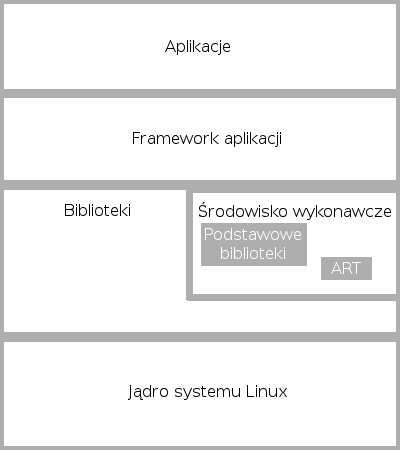
\includegraphics[width=0.5\linewidth]{02/warstwy_android}
	\end{center}
	\caption{Schemat architektury systemu Android}
\end{figure}

\subsubsection*{Środowisko wykonawcze}
Uruchamianiem programów napisanych w Javie zajmuje się wirtualna maszyna Javy (ang. Java Virtual Machine). Po skompilowaniu tworzony jest kod bajtowy, plik class, który następnie po załadowaniu interpretowany jest przez JVM (możliwa też kompilacja JIT). Takie podejście pozwala na przenośność programów, czyli niezależność od platformy, kosztem pewnego spadku wydajności.

Mimo, że programy na Androida pisane są w Javie, to nie JVM używany jest do ich późniejszego wykonywana. Głównie jest to spowodowane chęcią stworzenia środowiska uruchomieniowego, które będzie lepiej przystosowane do słabszych wydajnościowo od komputerów maszyn, jakimi są urządzenia mobilne. Proces budowania aplikacji rozpoczyna się tak samo. Kompilator przekształca pliki zawierające kod Javy, do kodu bajtowego. W takiej postaci program nie mógłby zostać jeszcze uruchomiony. Najpierw specjalne narzędzie, pod nazwą dx, modyfikuje wynik działania kompilatora. Jego zadaniem jest połączenie wszystkich tych kodów bajtowych w jeden plik dex, z usunięciem powtarzających się symboli oraz zmianą znajdujących się tam instrukcji, na odpowiednie dla Androida. Dzięki temu skompilowany program będzie mniejszy oraz powinien działać szybciej. Ostatnim etapem budowania aplikacji jest stworzenie pliku apk, odpowiednika jar, w którym oprócz kodu bajtowego, znajdą się takie zasoby jak zdjęcia wykorzystywane w aplikacji.

\begin{figure}[h]
	\begin{center}
		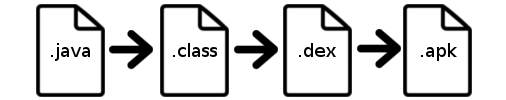
\includegraphics[width=0.5\textwidth]{02/android_dex}
	\end{center}
	\caption{Proces budowy aplikacji}
	\vspace{-0.5cm}
\end{figure}

Do wersji 4.4 Androida (KitKat) aplikacje uruchamiane były w wirtualnej maszynie Dalvik. Sposób działania jest dość zbliżony do JVM. Kod bajtowy w postaci plików dex jest interpretowany, z możliwością kompilacji do kodu natywnego (JIT). Jedną z różnic jest sposób działania wirtualnego procesora, który w Dalviku opartu został na rejestrach, a nie na stosie. Takie podejście wpływa na mniejsze zużycie pamięci, jednak programy są większe, gdyż instrukcje muszą zawierać dodatkowe informacje co do rejestrów, z których korzystają.

W wersji 5.0 Androida (Lolipop) zastąpiono dotychczasową maszynę wirtualną Dalvik, środowiskiem uruchomieniowym Android runtime (ART). Również przyjmuje pliki dex, jednak nie interpretuje ich, a w momencie instalacji aplikacji - kompiluje. Taka kompilacja kodu pośredniego, języka wysokiego poziomu, do kodu natywnego, nosi nazwę Ahead-of-time (AOT). Przy każdym uruchomieniu aplikacji, dzięki ART, wykorzystywany jest jej natywny kod. Ta zmiana powoduje szybsze działanie i uruchamianie się aplikacji. Wadą jest znacznie dłuższy czas instalacji, który teraz obejmuje także dodatkową kompilację.

\subsubsection*{Programowanie aplikacji}
Aby móc tworzyć aplikacje na Androida z wykorzystaniem Javy, konieczne jest posiadanie:

\begin{itemize}
	\item Java z JDK i JRE,
	\item Android SDK.
\end{itemize}

W ten sposób aplikacja do funkcji systemowych odwoływać się będzie za pomocą udostępnionego przez system API, przeznaczonego dla Javy. Dzięki temu, że nie jest to kod natywny, nie jest konieczna osobna kompilacja dla każdej dostępnej architektury. Programy są uniwersalne i dopiero po zainstalowaniu na konkretnym urządzeniu interpretowany jest kod bajtowy, bądź przeprowadzana kompilacja AOT. Przez twórców systemu udostępniane jest NDK, czyli Native Development Kit. Z jego pomocą aplikacje mogą być tworzone w C lub C++, odwołując się bezpośrednio do bibliotek systemowych. Niestety, mimo możliwego zysku na wydajności, stworzony kod jest zależny od architektury. Dodatkowo większość zewnętrznych bibliotek jest tworzonych w Javie. 

Bardzo zalecane jest używanie zintegrowanego środowiska programistycznego, które automatyzuje niektóre czynności. Potrafi stworzyć za użytkownika projekt z wymaganą strukturą plików, wykonać wszystkie etapy kompilacji, wgrać program na urządzenie i wiele innych. Dedykowanym IDE jest Android Studio, do niedawna wykorzystywany był domyślnie Eclipse.

\begin{figure}[h]
	\begin{center}
		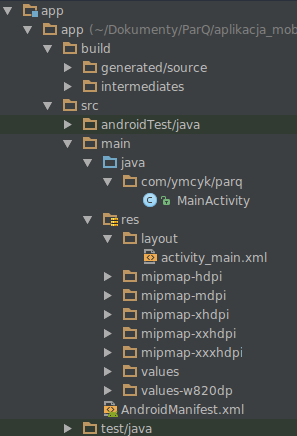
\includegraphics[width=0.25\textwidth]{02/android_pliki}
	\end{center}
	\caption{Pliki projektu utworzonego w Android Studio}
	\vspace{-0.3cm}
\end{figure}

Podczas działania aplikacja prezentuje użytkownikowi tzw. ekrany. Są to odpowiedniki okien systemowych, gdzie umieszczane są elementy graficznego interfejsu użytkownika, czyli widoki (ang. views), jak np.: przyciski, rozwijane listy, czy pola tekstowe. Wchodząc z nimi w interakcję, możliwa jest komunikacja między użytkownikiem, a urządzeniem. 

Wygląd ekranów definiowany jest w plikach XML, nazywanych układami (ang. layout). Każdy z widoków jest osobnym znacznikiem, a za pomocą argumentów można modyfikować wybrane parametry jak rozmiar, czy kolor. Wszystkie widoki w pliku XML muszą posiadać swojego rodzica, który definiuje jak mają one być traktowane w tym układzie. W Androidzie dostępnych jest ich kilka, a do najpopularniejszych należą: RelativeLayout (położenie widoków określane jest względem siebie), LinearLayout (układ liniowy, gdzie elementy GUI wyświetlane są jeden koło drugiego) i GridLayout (dzieli ekran na siatkę, składającą się z wierszy oraz kolumn, i pozwala umieścić widoki we wskazanych komórkach).

Układy definiują jak dany ekran ma wyglądać, natomiast aktywności (ang. activity), czyli klasy Javy, określają w jaki sposób mają one reagować na interakcje użytkownika. Przechodząc do danego ekranu, tworzona jest najpierw aktywność. W metodzie onCreate, wywoływanej przed wyświetleniem ekranu, wybierany jest układ, który ma zostać użyty przez system do stworzenia interfejsu. Widoki z tego układu mogą mieć powiązane ze sobą jakieś operacje, które będą przeprowadzane np.: po naciśnięciu przycisku. To także odbywa się w aktywności, która może posiadać metody wywoływane po zakończeniu danej interakcji.

Rozwiązania mobilne cieszą się coraz większym zainteresowaniem. Tylko w sklepie z aplikacjami Androida, Google Play, liczba programów przekroczyła w 2015 r. 1,6 mln \cite{biblia_ebiznesu_2}. Powstające coraz to nowe urządzenia, na których zainstalowany jest Android sprawia, że umiejętność programowania na tą platformę będzie coraz bardziej doceniana.


\subsection{Framework Django}
Frameworki aplikacji internetowych powstały z myślą o zwolnieniu programisty z obowiązku pisania części kodu, który jest wspólny dla większości serwisów. Może to być dostęp do bazy danych, obsługa linków (ang.~routing), czy zarządzanie sesjami. Dodatkowo, pisanie aplikacji internetowej od podstaw, jest zadaniem czasochłonnym oraz dość trudnym. Frameworki są odpowiedzią na te problemy, dostarczając zestaw gotowych oraz przetestowanych rozwiązań, które należy dostosować do własnych potrzeb. Umożliwiają utworzenie struktury plików projektu, na bazie którego dalej będzie rozwijana aplikacja. Każdy z najpopularniejszych języków programowania oferuje duży wybór silników, przeznaczonych do tworzenia usług internetowych i np.: w C\# napisane zostały ASP.NET i MonoRail, w Javie - Spring i JavaServer Faces, a w Python - Django i Flask. Mogą się różnić przede wszystkim stopniem złożoności, dzięki czemu nadają się do różnych zastosowań - prezentują odmienne sposoby realizacji podobnych zadań. Wybór programisty będzie głównie zależny od jego prywatnych preferencji.

\subsubsection*{Początki Django}
Django rozwijany jest jako wolne oprogramowanie na GitHub'ie, w ramach fundacji Django Software Foundation, ale skupiaja wokół siebie także wielu niezależnych twórców. Został napisany w Pythonie, stając się z czasem najpopularniejszym frameworkiem dla tego języka. Jego historia rozpoczęła się w 2003~r., kiedy to dwóch programistów Adrian Holovaty i Simon Willison zaczęli używać Pythona do tworzenia aplikacji webowych dla kilku serwisów informacyjnych, m.in. Lawrence.com. Praca w środowisku dziennikarskim, cechująca się napiętym grafikiem, wymagała niezwykle szybkiej realizacji zadań. Z tej konieczności opracowali własny silnik, który w 2005~r., już pod nazwą Django, został udostępniony publicznie. To właśnie szybkość oraz względna łatwość tworzenia aplikacji są jego głównymi zaletami.

\subsubsection*{Charakterystyka}

Aplikacje Django tworzone są w interpretowanym języku Python, przeznaczonym głównie do pisania skryptów. Jako że jego interpretery dostępne są na wielu platformach, jest on niezależny od systemu operacyjnego. Dodatkowo wsparcie do wielu paradygmatów (imperatywnego, funkcyjnego, obiektowego), przekłada się na jego szerokie zastosowanie. Oprócz programowania serwerów, jest używany do pisania testów, aplikacji z graficznym interfejsem, a także gier 3D. Wyróżnia się głównie charakterystyczną składnią, w której poszczególne bloki kodu odseparowane są wcięciami (spacje lub tabulator). Wpływa to na zwiększoną czytelność kodu.

Architektura aplikacji sieciowych typu klient-serwer, opiera się często na wzorcu projektowym Model-View-Controller (pol.~Model-Widok-Kontroler), w skrócie MVC. Jego ideą jest odseparowanie części prezentacji danych, od kodu odpowiedzialnego za ich przetwarzanie. Aplikacja dzielona jest w nim na trzy główne części. Model jest reprezentacją danych oraz logiki problemu. Widok odpowiedzialny jest za prezentację - określa w jaki sposób informacje mają zostać przedstawione. Kontroler przyjmuje żądania i wykonuje związane z nimi akcje. Głównie aktualizuje widoki oraz modele.

\begin{figure}[h]
	\begin{center}
		\includegraphics[width=0.6\textwidth]{02/MVC_diagram}
	\end{center}
	\caption{Wzorzec projektowy MVC}
	\vspace{-0.3cm}
\end{figure}

Wzorzec MVC jest stosowany w Django, jednak został zrealizowany w sposób odmienny od najczęściej spotykanych jego implementacji. Z tego względu często nazywa się go wzorcem MTV (Model-Template-View), będącego pewną wariacją MVC. Także wyróżnia się w nim trzy główne części aplikacji, a są to:
\begin{itemize}
	\item Model -- podobnie jak w MVC, zapewnia dostęp do danych. Opisane są tutaj relacje między danymi oraz odbywa się ich walidacja.
	\item Template (pol. szablon) -- warstwa prezentacji, czyli jak ma zostać wygenerowana odpowiedź (w postaci dokumentu HTML lub innym formacie).
	\item View (pol. widok) -- zawiera logikę biznesową. Pobiera dane z modeli i łączy je z szablonami, tworząc w ten sposób odpowiedź. Stanowi pomost między dwoma wcześniej wymienionymi elementami MTV.
\end{itemize}
Rolę kontrolera MVC pełni w Django sam framework. Otrzymane zapytanie wysyłane jest do odpowiedniego widoku, w zależności od konfiguracji URL.

\begin{singlespace}
	\captionof{listing}{Przykładowa konfiguracja URL w Django}
	\vspace{0.3cm}
	\inputminted[fontsize=\footnotesize]{python}{src/urls.py}
	\label{l:url}
\end{singlespace}

% tutaj o wszystkich cechach Django
W przeciwieństwie do mikro frameworków, takich jak Flask, Django dostarcza programiście wielu gotowych rozwiązań, jak: dostęp do baz danych, klasy ORM, obsługa linków URL, uprawnienia użytkowników, automatycznie generowana strona administratora, szablony HTML i wiele innych. Dodatkowo posiada wbudowaną ochronę przed typowymi atakami, takimi jak: cross-site scripting (XSS), cross-site request forgery (CSRF), a także wstrzykiwanie SQL'a.

\subsubsection*{Programowanie aplikacji}
Tak jak większość frameworków, także i Django tworzy za użytkownika gotową strukturę projektu. Poza konfiguracją, nie znajduje się w nim jednak żadna logika. Wszystkie modele oraz widoki w danym projekcie tworzone są w ramach tzw. aplikacji, czyli pakietów Pythona (których struktura także generowana jest przez framework), odpowiednio w plikach models.py oraz views.py. Dzięki temu mogą zostać one ponownie wykorzystane. W hierarchii plików znajdują się na tym samym poziomie, co projekt. 

\begin{figure}[h]
	\begin{center}
		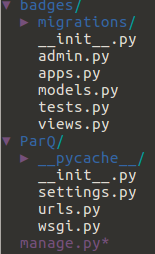
\includegraphics[width=0.15\textwidth]{02/django_structuree}
	\end{center}
	\caption{Struktura plików projektu (ParQ) z aplikacją (badges)}
	\vspace{-0.3cm}
\end{figure}

W pliku settings.py projektu znajdują się wszystkie ustawienia serwisu, takie jak konfiguracja bazy danych, strefy czasowej, silnika szablonów oraz pakietów pośredniczących (middleware) wykorzystywanych np.: do autoryzacji. Tam także powinny zostać zarejestrowane wszystkie aplikacje używane w projekcie.

W models.py aplikacji znajdują się modele danych - są to klasy dziedziczące po Model. Posiadają zmienne klasowe, które reprezentują kolumny w tabelach baz danych. Nazwa takiego pola jest później używana jako nazwa kolumny, natomiast jej typ definiowany jest przez instancję jednej z klas pochodnych od Field. I tak dla przykładu IntegerField będzie typem całkowitoliczbowym, a CharField znakowym. Parametry podane w konstruktorze pozwalają zdefiniować rozmiar, czy unikalność krotki w kolumnie. Relacje również tworzone są za pomocą pól. Model posiadający pole relacji, może odwoływać się za jego pomocą do powiązanych danych. W Django znajdują się trzy takie klasy:

\begin{itemize}
	\item ForeignKey -- pole z kluczem obcym, używane w relacjach jeden do wielu. Tworzona jest kolumna w tabeli.
	\item ManyToManyField -- używane w relacjach wiele do wielu. W bazie danych zostanie automatycznie utworzona tabela pośrednia, z kluczami powiązanych tabel.
	\item OneToOneField -- do relacji jeden do jeden. Także wykorzystywana jest tabela pośrednia, jednakże oba klucze są unikalne - mogą wystąpić tylko w jednej relacji w ramach tej tabeli.
\end{itemize}

W modelach dozwolone jest także definiowanie własnych metod.

\begin{singlespace}
	\captionof{listing}{Przykładowy model danych z modułu models.py}
	\vspace{0.3cm}
	\inputminted[fontsize=\footnotesize]{python}{src/models.py}
\end{singlespace}

Kolejnym ważnym plikiem w aplikacji tworzonej przez użytkownika jest views.py. To tutaj znajdują się widoki ze wzorca MTV i scalają one szablony z modelami. Jako parametr przyjmują obiekt HttpRequest, zawierający dane zawarte w żądaniu HTTP. To właśnie te widoki podawane są podczas konfiguracji linków w funkcji url, pliku urls.py w projekcie. Zostało to zaprezentowane na listingu \ref{l:url}.

\begin{singlespace}
	\captionof{listing}{Widok}
	\vspace{0.3cm}
	\inputminted[fontsize=\footnotesize]{python}{src/views.py}
\end{singlespace}

\subsubsection*{Aplikacje jako dodatki}
Napisane aplikacje Django, mogą być wielokrotnie wykorzystywane w innych projektach. Na tej zasadzie funkcjonują dodatki pisane do tego frameworku. Jednymi z nich są: Django REST Framework używany do tworzenia API w architekturze REST, czy django-annoying modyfikujący działanie niektórych elementów silnika.


		\newpage
		
		%\section{Podobne rozwiązania}
		%\newpage
		
		\section{Projekt systemu}
\subsection{Wymagania funkcjonalne}
\subsection{Wymagania niefunkcjonalne}
\subsection{Diagramy UML}
\subsection{Projekt bazy danych}
		\newpage
		
		\setcounter{listing}{0}

\section{Implementacja systemu}

W tym rozdziale zawarte są szczegóły implementacji systemu dla wybranych funkcjonalności, do przedstawienia których posłużono się fragmentami kodów źródłowych. Następnie na zrzutach ekranu zaprezentowane zostały wyniki działania systemu. Koniec rozdziału poświęcony został sposobom testowania, a także opisowi wykorzystanych środowisk programistycznych i edytorów kodu.

\subsection{Aplikacja internetowa}

Do głównych zadań serwera należą: autoryzacja, zarządzanie i identyfikowanie pojazdów, kupno oraz kontrola biletu postojowego. Wszystkie funkcjonalności udostępniane są aplikacji mobilnej poprzez API w postaci adresów URL. Wysyłając żądanie na jeden z nich, aplikacja otrzyma w odpowiedzi dokument JSON. W Django, czyli frameworku użytym do implementacji części serwerowej systemu, miejscem przeznaczonym do mapowania adresu na widok jest plik urls.py. Jego fragment został zaprezentowany na listingu \ref{parq_urls}. W tym miejscu znajdują się także wszystkie adresy w systemie, na jakie aplikacja mobilna będzie wysyłać swoje żądania.

\begin{singlespace}
	\captionof{listing}{Mapowane adresy URL z pliku urls.py.}
	\label{parq_urls}
	\vspace{0.3cm}
	\inputminted[fontsize=\footnotesize, linenos=true]{python}{src/imp/urlpatterns.py}
\end{singlespace}

\subsubsection*{Tworzenie konta i autoryzacja}

Z procesem utworzenia konta w systemie przez kierowcę i kontrolera związanych jest kilka dodatkowych czynności, którymi są przypisanie roli oraz generowanie tokenu autoryzacyjnego. Wszyscy użytkownicy tworzeni są w oparciu o istniejący już w Django model użytkownika -- User, z modułu django.contrib.auth.models. Niezbędny jest jednak sposób, który pozwoli na odróżnienie kont kierowcy i kontrolera, aby można było nadać im odmienne uprawnienia. Do tego celu wykorzystany został dodatek djroles, napisany specjalnie na potrzeby tego systemu. Swoje działanie opiera na istniejących w Django grupach, z którymi domyślnie użytkownicy są w relacji wiele-do-wielu, czyli mogą należeć do kilku grup jednocześnie. Jego zadaniem jest umożliwienie wybrania zestawu grup, spośród których użytkownik może należeć tylko do jednej w tym samym czasie. Do tego celu tworzona jest tabela pomocnicza -- Role, w której umieszczane będą grupy, nazywane dalej rolami. Na listingu \ref{driver} pokazany został sposób, w jaki deklarowane są grupy, które będą używane do tworzenia ról. Jest to robione poprzez napisanie klasy Pythona, która dziedziczy po BaseRole - nazwa utworzonej roli będzie pokrywać się z nazwą klasy. Dzięki możliwemu wielodziedziczeniu w tym języku, do tego celu mogą zostać wykorzystane zdefiniowane wcześniej modele.

\begin{singlespace}
	\captionof{listing}{Fragment modelu Driver.}
	\label{driver}
	\vspace{0.3cm}
	\inputminted[fontsize=\footnotesize, linenos=true]{python}{src/imp/driver.py}
\end{singlespace}

\vspace{0.3cm}

Poza przypisaniem grupy, każdy użytkownik w systemie, niezależnie już od pełnionej roli, musi posiadać wygenerowany token autoryzacyjny. Obie te czynności muszą zostać wykonane w momencie utworzenia konta. Zostało to zrealizowane poprzez sygnały (ang. signals) dostępne w Django. Są to funkcje, które zostaną wykonane w odpowiedzi na jakieś zdarzenie związane z ustaloną klasą w projekcie. Na listingu \ref{sygnaly} przedstawione zostały sygnały powiązane z domyślną klasą użytkownika User (tworzenie tokenu) oraz klasami Driver i Officer (przypisywanie do ról). Wykonywane są w odpowiedzi na zapisanie modelu w bazie danych, czyli sygnał post\_save.

\begin{singlespace}
	\captionof{listing}{Sygnały związane z tworzeniem konta w systemie.}
	\label{sygnaly}
	\vspace{0.3cm}
	\inputminted[fontsize=\footnotesize, linenos=true]{python}{src/imp/token_signal.py}
\end{singlespace}

\subsubsection*{Identyfikacja pojazdów}

Z każdym pojazdem kierowcy w systemie powiązany jest identyfikator UUID (ang. Universally unique identifier), czyli 128-bitowa losowa wartość. Przechowywana jest ona w modelu Badge (listing \ref{model_badge}), powiązanym relacją jeden-do-jeden z pojazdem (Vehicle). W modelu znajduje się także metoda generate\_image(), która odpowiedzialna jest za generowanie kodu QR, w którym zakodowany będzie identyfikator. W niej wykorzystywane są funkcje pochodzące z zewnętrznej biblioteki Pythona -- qrcode. Oprócz danych, podawany jest także poziom korekcji błędów i wersja kodu.

\begin{singlespace}
	\captionof{listing}{Badge - model identyfikatora.}
	\label{model_badge}
	\vspace{0.3cm}
	\inputminted[fontsize=\footnotesize, linenos=true]{python}{src/imp/badges-badge.py}
\end{singlespace}

\vspace{0.3cm}

Utworzony w ten sposób kod QR jest następnie wysyłany na e-maila podanego przez kierowcę podczas rejestracji. Umieszczony w widocznym miejscu pojazdu, będzie skanowany przez kontrolera podczas sprawdzania biletu.

\subsubsection*{Taryfikator}

Taryfikator oprócz powiązanych ze sobą opłat, musi zawierać także informację o czasie w którym obowiązuje. Taką możliwość daje klasa Event, pochodząca z dodatku django-scheduler. Pozwala ona na stworzenie wydarzenia z datą początkową oraz końcową, a dzięki klasie Rule, istnieje możliwość jego powtarzania np.: co tydzień. Model Schedule rozszerza Event, dzięki czemu  przetrzymuje informacje zarówno o opłatach, jak i czasie swojego obowiązywania. Dzięki możliwości tworzenia wydarzeń cyklicznych, może zostać ustawiony na wybrany dzień tygodnia. Na listingu \ref{schedule-create} przedstawiono przykład jego tworzenia.

\begin{singlespace}
	\captionof{listing}{Tworzenie cotygodniowego taryfikatora.}
	\label{schedule-create}
	\vspace{0.3cm}
	\inputminted[fontsize=\footnotesize, linenos=true]{python}{src/imp/schedule-create.py}
\end{singlespace}


\subsubsection*{Kupno biletu}

Za obliczenie kosztu biletu odpowiedzialne są fragmenty kodu przedstawione na listingach \ref{calculate-schedule} i \ref{calculate-charge}. Bazują na zasadzie naliczania opłaty stosowanej w szczecińskiej Strefie Płatnego Parkowania, w której stawki zmieniają się w zależności od długości postoju. W klasie Schedule obliczany jest najpierw czas trwania parkowania w minutach. Następnie po pobieraniu wszystkich opłat, w pętli każda z nich nalicza swoją część ceny (model Charge) zgodnie z jej czasem obowiązywania. W przypadku wyczerpania listy opłat przed zakończeniem postoju, ostatnia z nich (tak jak w SPP w Szczecinie) naliczy cenę dla pozostałych minut postoju. W pętli wszystkie opłaty cząstkowe są sumowane, wyznaczając w ten sposób koszt biletu.

\begin{singlespace}
	\captionof{listing}{Obliczanie łącznej kwoty w klasie Schedule.}
	\label{calculate-schedule}
	\vspace{0.3cm}
	\inputminted[fontsize=\footnotesize, linenos=true]{python}{src/imp/schedule-calculate_price.py}
\end{singlespace}

\begin{singlespace}
	\captionof{listing}{Obliczanie częstki ceny w pojedynczej opłacie - model Charge.}
	\label{calculate-charge}
	\vspace{0.3cm}
	\inputminted[fontsize=\footnotesize, linenos=true]{python}{src/imp/charge-calculate_price.py}
\end{singlespace}

\vspace{0.3cm}

Obliczanie opłaty za postój następuje w momencie kupowania biletu, po czym portmonetka użytkownika zostanie obciążona odpowiednią kwotą. Jeśli nie posiada on wystarczającej ilości pieniędzy, bilet nie może zostać kupiony.

\subsubsection*{Doładowanie konta}

%TODO sprawdzaj czy podane linie się zgadzają!
Doładowywanie konta odbywa się dwuetapowo. Najpierw w aplikacji mobilnej użytkownik przelewa pieniądze za pomocą bramki płatności PayPal. W przypadku powodzenia transakcji zwrócony zostanie jej identyfikator, który wysyłany jest do serwera systemu ParQ. Na listingu \ref{payments_list} przedstawiony został widok odpowiedzialny za to żądanie. W linii 12 wywoływana jest metoda, w której otrzymany od aplikacji mobilnej identyfikator, przesyłany zostaje do serwera PayPal'a, celem uzyskania informacji o kwocie jaka została przelana. Następnie jeśli wszystko się zgadza, numer transakcji zapisywany jest w bazie danych (linia 13). Gdyby transakcja o takim identyfikatorze już istniała, doładowywanie zostanie przerwane. Tylko w razie powodzenia wykonany będzie dalszy fragment kodu, gdzie powiązana portmonetka użytkownika jest uzupełniana o wpłaconą kwotę.

\begin{singlespace}
	\captionof{listing}{payment\_list - widok doładowania konta użytkownika.}
	\label{payments_list}
	\vspace{0.3cm}
	\inputminted[fontsize=\footnotesize, linenos=true]{python}{src/imp/paypal-views.py}
\end{singlespace}

\vspace{0.3cm}
%TODO pamiętać, żeby było razem z tym na dole
Do realizacji tej części pracy wykorzystano kilka dodatków do Django oraz jeden dodatkowy pakiet Pythona, a są to:

\begin{itemize}
	\item Django REST Framework -- na jego podstawie tworzone są widoki, które obsługują żądania w architekturze REST. Ten dodatek umożliwia także autoryzacje żądań, opartą na generowanym wcześniej tokenie.
	\item django-scheduler -- tworzenie wydarzeń, które mogą się powtarzać cyklicznie.
	\item django-ordered-model -- numerowane relacje w tabelach.
	\item django-countries -- państwa i ich kody ze standardu ISO 3166.
	\item djroles -- tworzenie ról w Django.
	\item qrcode -- pakiet Pythona umożliwiający generowanie kodów QR.
\end{itemize}

\subsection{Aplikacje mobilne}

W ramach pracy zostały wykonane dwie oddzielne aplikacje mobilne -- dla kierowcy oraz kontrolera. Kierowca oprócz logowania, może założyć konto, czy dokonać płatności celem doładowywania portmonetki. Kontroler w swojej aplikacji może skanować plakietki z kodem QR, aby przeprowadzić kontrolę biletu. Do każdej z tych aplikacji zalogować może się jedynie użytkownik posiadający konto, do którego została przypisana odpowiednia rola. Obie wymagają ciągłej komunikacji z serwerem.

\subsubsection*{Parsowanie danych}

Format JSON jest obecnie najpopularniejszym formatem, wykorzystywanym do wymiany danych w architekturze REST. Wszystkie dane to zmienne, a ich nazwy są otoczone cudzysłowami. Wartości mogą być typu string (ciąg znaków), liczbami całkowitymi i zmiennopozycyjnymi, a także tablicami w których skład wchodzą wymienione wyżej zmienne, bądź obiektem JSON. Obiekty i tablice nie mają żadnych ograniczeń, jeśli chodzi o ich zagnieżdżanie. W celu wydobycia informacji, JSON musi być poddany odpowiedniej analizie, zarówno na serwerze jak i aplikacji mobilnej. W Androidzie parsowanie można wykonać za pomocą klas JSONObject oraz JSONArray z pakietu org.json. Ta druga służy do analizy tablic danych. 
\\
\\
JSONObject umożliwia parsowanie pojedynczego JSONa, a dane do analizy podawane są jako ciąg znaków (String) w konstruktorze. Metody tej klasy służące do wydobywania wartości, jako parametr przyjmują nazwę klucza z którym ta wartość jest związana. Są to m.in get(), getInt(), czy getString(), a ich użycie zależy od spodziewanego typu wartości przechowywanego w dokumencie. Istnieje także metoda getJSONObject(), która zwraca zagnieżdżony obiekt JSONa w postaci instancji klasy JSONObject. JSONArray instancjonowana jest w podobny sposób. Po wywołaniu metody getJSONObject() z indeksem elementu w parametrze, zwracany jest obiekt pojedynczego JSONa, czyli klasy JSONObject. Na listingu \ref{parsowanie} znajduje się przykład z wykorzystaniem kolekcji danych.

\newpage

\begin{singlespace}
	\captionof{listing}{Parsowanie jsona dla kolekcji pojazdów kierowcy.}
	\label{parsowanie}
	\vspace{0.3cm}
	\inputminted[fontsize=\footnotesize, linenos=true]{java}{src/imp/parsowanie-json.java}
\end{singlespace}

\vspace{0.3cm}

Ten fragment kodu zostaje wykonany w momencie otrzymania z serwera listy pojazdów powiązanych z danym kierowcą. Dla każdego elementu tablicy JSON wydobywany jest obiekt klasy JSONObject, z którego pobierane są dane pojazdu. Zostają one później zaprezentowane użytkownikowi w odpowiednim widoku.

\subsubsection*{Komunikacja z serwerem}

Komunikacja w systemie polega na wysyłaniu żądań przez aplikacje do serwera i oczekiwaniu na rezultat, który zostanie przesłany w odpowiedzi. Tym zajmuje się biblioteka do komunikacji HTTP -- Volley. Stanowi alternatywę dla wykorzystywanych wcześniej klas Javy, jak HttpURLConnection, będąc rozwiązaniem dedykowanym dla Androida, cechującym się prostotą i szybkością działania. Świetnie nadaje się do prostych API, w których wymiana informacji polega na przesyłaniu list oraz pojedynczych danych w formacie JSON. Jedną z jej głównych zalet jest zdolność do buforowania odpowiedzi. Jeśli zapytanie może zostać obsłużone dzięki danym znajdującym się w pamięci podręcznej, nie będzie ono musiało zostać ponownie wysłane.
\\
\\
Listing \ref{volley} przedstawia sposób, w jaki konstruowane są zapytania w tej bibliotece. Najpierw w konstruktorze podawany jest rodzaj metody HTTP oraz adres, na jaki żądanie ma zostać wysłane. Dwa następne parametry to obiekty klas anonimowych. Jeśli odpowiedz z serwera będzie zwrócona z kodem HTTP oznaczającym powodzenie operacji (2xx), to wykonana zostanie metoda onResponse() pierwszego obiektu. Parametr response zawiera dane odpowiedzi i to właśnie on będzie poddawaniu parsowaniu. Jeśli odpowiedz jest błędna, czyli wysłana została z kodem błędu (4xx lub 5xx), wywołana będzie onErrorResponse(). Tak utworzone zapytanie dodawane jest do kolejki zapytań, w której moment wysłania zależy od priorytetu jaki został nadany.

\begin{singlespace}
	\captionof{listing}{Wysłanie żądania.}
	\label{volley}
	\vspace{0.3cm}
	\inputminted[fontsize=\footnotesize, linenos=true]{java}{src/imp/scan-activity.java}
\end{singlespace}

\subsubsection*{Realizacja płatności}

Do integracji PayPal'a z aplikacją mobilną została wykorzystana biblioteka PayPal Android SDK, która jest dostępna w na licencji open source. Razem z nią, oprócz możliwości realizacji opłat, udostępniane są także gotowe ekrany dla aplikacji mobilnej, na których użytkownik może podać swoje dane uwierzytelniające. Biblioteka ta pozwala na realizowanie płatności pojedynczych (tzw. Single Payment, użytkownik za każdym razem musi podawać dane uwierzytelniające) oraz automatycznych (Future Payment, dane podawane tylko raz, a zwrócony token OAuth pozwala na dokonywanie płatności w imieniu użytkownika). W tworzonym systemie oferowana jest tylko pierwsza opcja.
\\
\\
Na listingu \ref{paypal1} przedstawiony został fragment, w którym za pomocą intencji uruchomiona zostaje aktywność uwierzytelnienia płatności. W klasie PayPalPayment podawane zostają informacje odnośnie wysokości płatności, waluty oraz typu transakcji. Obiekt tej klasy, razem z informacjami konfiguracyjnymi, zostaje umieszczony w intencji. Wywołanie metody aktywności Androida startActivityForResult() spowoduje wyświetlenie nowego ekranu.

\begin{singlespace}
	\captionof{listing}{Intencja rozpoczynająca aktywność PayPal'a.}
	\label{paypal1}
	\vspace{0.3cm}
	\inputminted[fontsize=\footnotesize, linenos=true]{java}{src/imp/get-payment.java}
\end{singlespace}

\vspace{0.3cm}

Metoda startAcitvityForResult() uruchamiająca nową aktywność różni się od startActivity() tym, że od docelowej aktywności oczekiwane jest otrzymanie jakiegoś wyniku. Po zakończeniu utworzonego ekranu uruchomiona zastanie metoda onActivityResult(). Do niej właśnie przesłana zostanie odpowiedź z serwera PayPal'a o statusie przeprowadzonej płatności, a także w razie sukcesu, identyfikator płatności. W tym miejscu właśnie będzie on wysłany do serwera systemu, celem jego dalszego uwierzytelnienia.

\subsubsection*{Kontrola biletu}

Kontrola biletu możliwa jest w aplikacji przeznaczonej dla kontrolera. Odbywa się poprzez skanowanie obrazu z kamery wbudowanej w urządzenie mobilne, do czego użyta została biblioteka ZXing ("Zebra Crossing"). Służy ona do przetwarzania obrazu, w celu odkodowania kodów graficznych QR i kreskowych. Domyślnie nie są dołączone do niej żadne gotowe aktywności jak w przypadku PayPal Android SDK, istnieje jednak dodatek -- ZXing Android Embedded, który takie dostarcza. Sposób działania jest dzięki niemu zbliżony do kroków, jakie należało wykonać podczas przeprowadzania transakcji. Zawiera on gotową aktywność, w której zostaje uruchomiona kamera urządzenia mobilnego. Na listingu \ref{platnosc} w klasie IntentIntegrator konfigurowany jest najpierw skaner, gdzie podawany jest rodzaj kodów graficznych jakich ma poszukiwać oraz orientacja ekranu. Po natrafieniu przez skaner na kod, skanowanie zostaje zakończone, a informacja jaką udało się odkodować zwracana jest w metodzie onActivityResult().

\begin{singlespace}
	\captionof{listing}{Intencja rozpoczynająca aktywność skanowania.}
	\label{platnosc}
	\vspace{0.3cm}
	\inputminted[fontsize=\footnotesize, linenos=true]{java}{src/imp/start-scan.java}
\end{singlespace}

\newpage

\subsection{Wyniki działania systemu}

Kierowca korzystający z systemu ParQ, oprócz logowania i rejestracji, może także doładować konto, dodawać nowe pojazdy oraz kupować bilety postojowe w przeznaczonej dla niego aplikacji. Kontroler natomiast ma możliwość przeprowadzenia kontroli zaparkowanego pojazdu. Poniżej znajduje się opis funkcjonującego systemu, z zrzutami ekranów z aplikacji mobilnych oraz wynikami działania serwera.
\\
\\
W pierwszej kolejności opisana została aplikacja przeznaczona dla kierowcy korzystającego ze strefy płatnego parkowania. Po zalogowaniu do niej, wyświetlany jest ekran główny, znajdujący się na rys. 5.1. To tutaj użytkownik uzyskuje podstawowe dane powiązane ze swoim kontem, takie jak ilość pieniędzy znajdujących się w portmonetce, czy godziny obowiązywania płatnego postoju. Tutaj też są wyświetlane informacje o wszystkich aktywnych biletach postojowych, wraz z informacjami o pojeździe na który zostały zakupione i godziną ich zakończenia. Z ekranu głównego możliwe jest przejście do pozostałych ekranów aplikacji. Po naciśnięciu ikonki w lewym górnym rogu, wysuwa się menu boczne przedstawione na rys. 5.2. Na górze wyświetlana jest nazwa oraz e-mail zalogowanego użytkownika. Poniżej znajdują się opcje przenoszące do ekranów zakupu biletu, zarządzania pojazdami lub doładowywania konta.

\begin{figure}[h]
	\centering
	\begin{minipage}[b]{0.25\textwidth}
		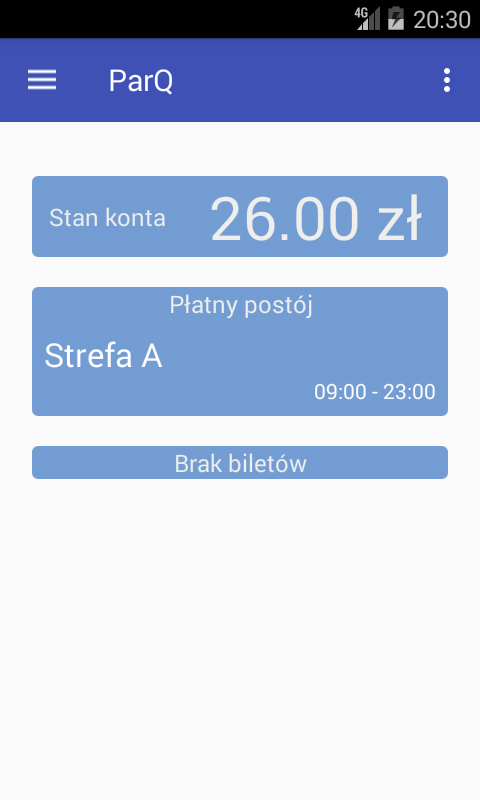
\includegraphics[width=\textwidth]{05/driver_dashboard3}
		\caption{Informacje o koncie.}
	\end{minipage}
	%\hfill
	\hspace{3cm}
	\begin{minipage}[b]{0.25\textwidth}
		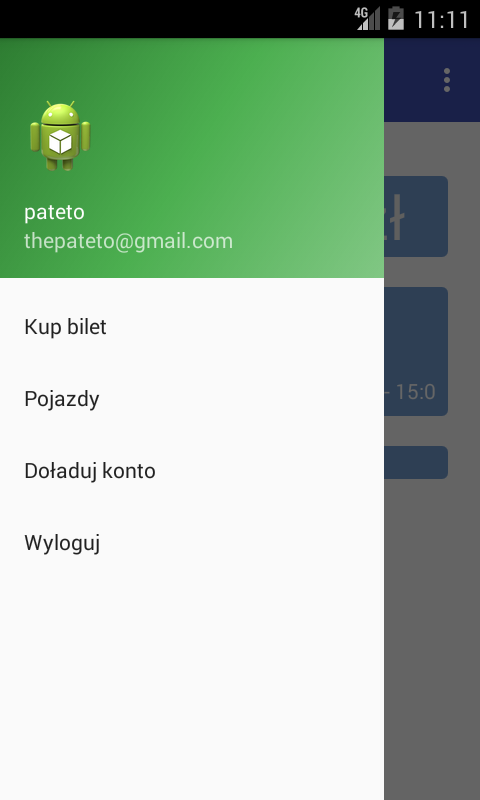
\includegraphics[width=\textwidth]{05/driver_drawer}
		\caption{Menu boczne aplikacji.}
	\end{minipage}
\end{figure}

Doładowywanie konta (rys. 5.3 i 5.4) rozpoczyna się od podania kwoty, jaką konto użytkownika w systemie ma zostać doładowane. Zatwierdzenie jej, powoduje pokazanie ekranów pochodzących z wykorzystywanej do realizacji płatności biblioteki -- PayPal Android SDK. Umożliwia ona wybranie metody płatności, uwierzytelnienie oraz zatwierdzenie transakcji. Po zakończeniu, użytkownik przenoszony jest na ekran główny, z zaktualizowanym stanem konta.

\newpage

\begin{figure}[h!]
	\centering
	\begin{minipage}[b]{0.25\textwidth}
		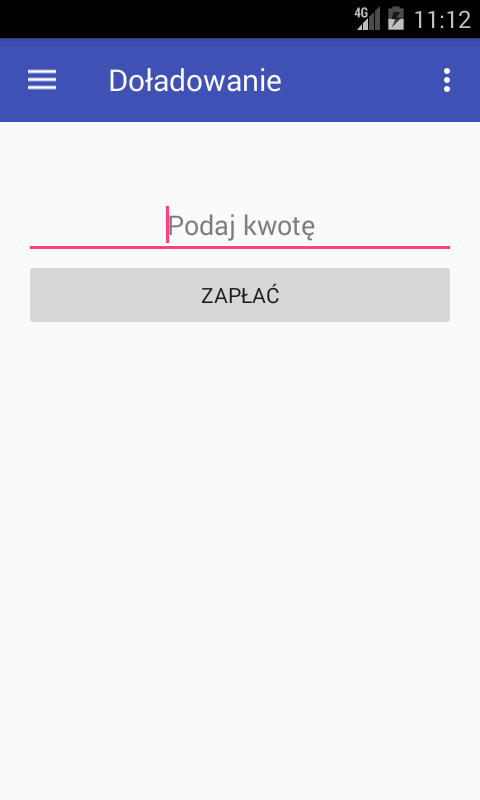
\includegraphics[width=\textwidth]{05/driver_doladowanie}
		\caption{Pole z kwotą doładowania.}
	\end{minipage}
	%\hfill
	\hspace{3cm}
	\begin{minipage}[b]{0.25\textwidth}
		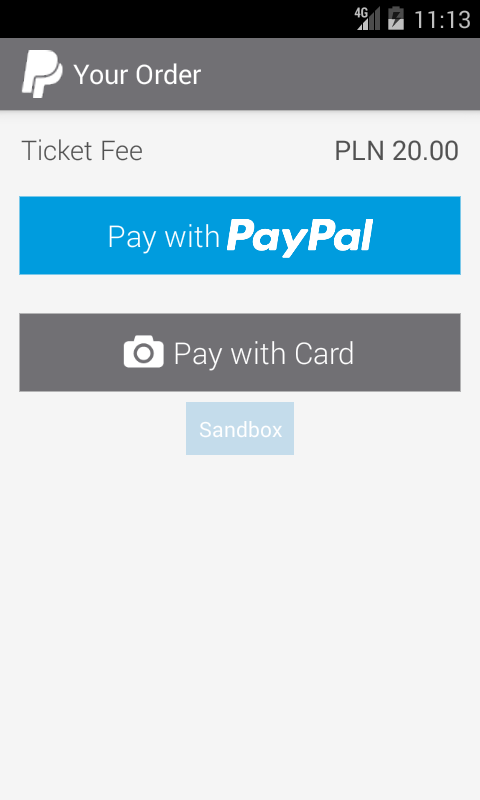
\includegraphics[width=\textwidth]{05/driver_paypal1}
		\caption{Realizacja płatności w PayPal.}
	\end{minipage}
\end{figure}

Do zakupu biletu w systemie niezbędna jest informacja o pojeździe oraz parkingu, w którym będzie odbywał się postój. Te czynności wykonywane są na dwóch ekranach zaprezentowanych poniżej. Wybranie samochodu na rys. 5.5 spowoduje wyświetlenie ekranu z rys. 5.6, gdzie należy wskazać parking oraz czas postoju w minutach. Gdy użytkownik posiada odpowiednią ilość pieniędzy, nastąpi zakupienie biletu, czego potwierdzenie znajdzie się na ekranie głównym aplikacji.

\begin{figure}[h!]
	\centering
	\begin{minipage}[b]{0.25\textwidth}
		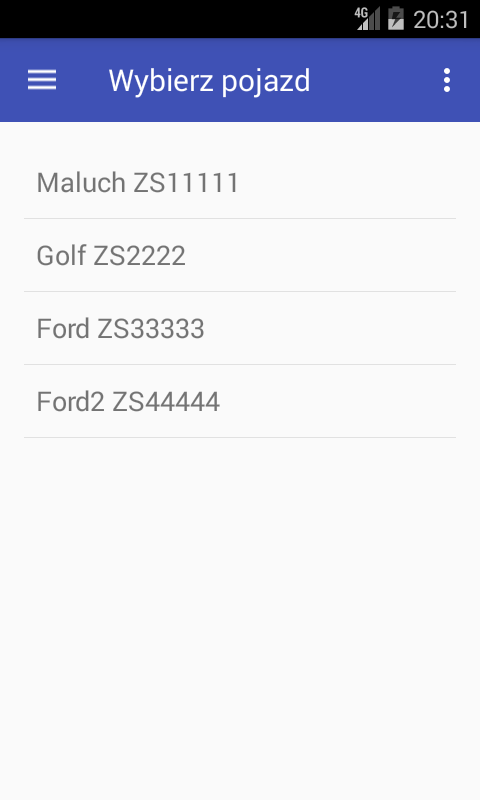
\includegraphics[width=\textwidth]{05/driver_kup_bilet1}
		\caption{Zakup biletu - wybór pojazdu.}
	\end{minipage}
	%\hfill
	\hspace{3cm}
	\begin{minipage}[b]{0.25\textwidth}
		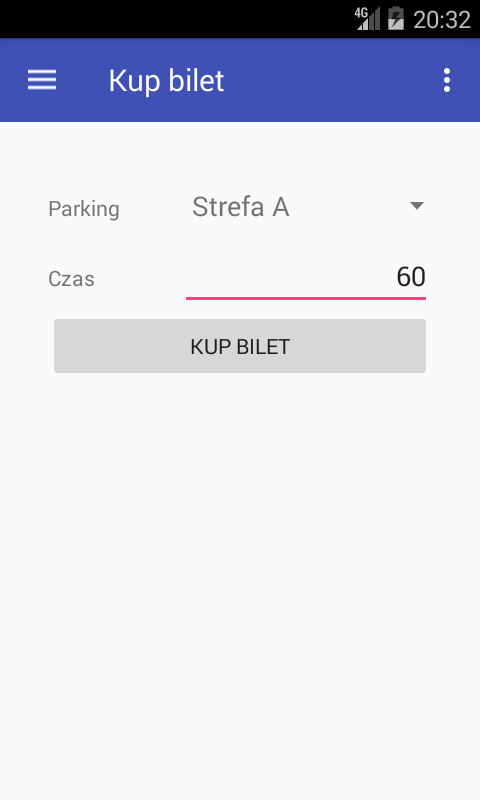
\includegraphics[width=\textwidth]{05/driver_kup_bilet2}
		\caption{Zakup biletu - parking i czas.}
	\end{minipage}
\end{figure}

Na rys. \ref{przejscia_kierowca} znajduje się schemat, na którym przedstawione zostały wszystkie ekrany oraz możliwe przejścia między nimi w aplikacji przeznaczonej dla kierowców.

\newpage

\begin{figure}[h!]
	\begin{center}
		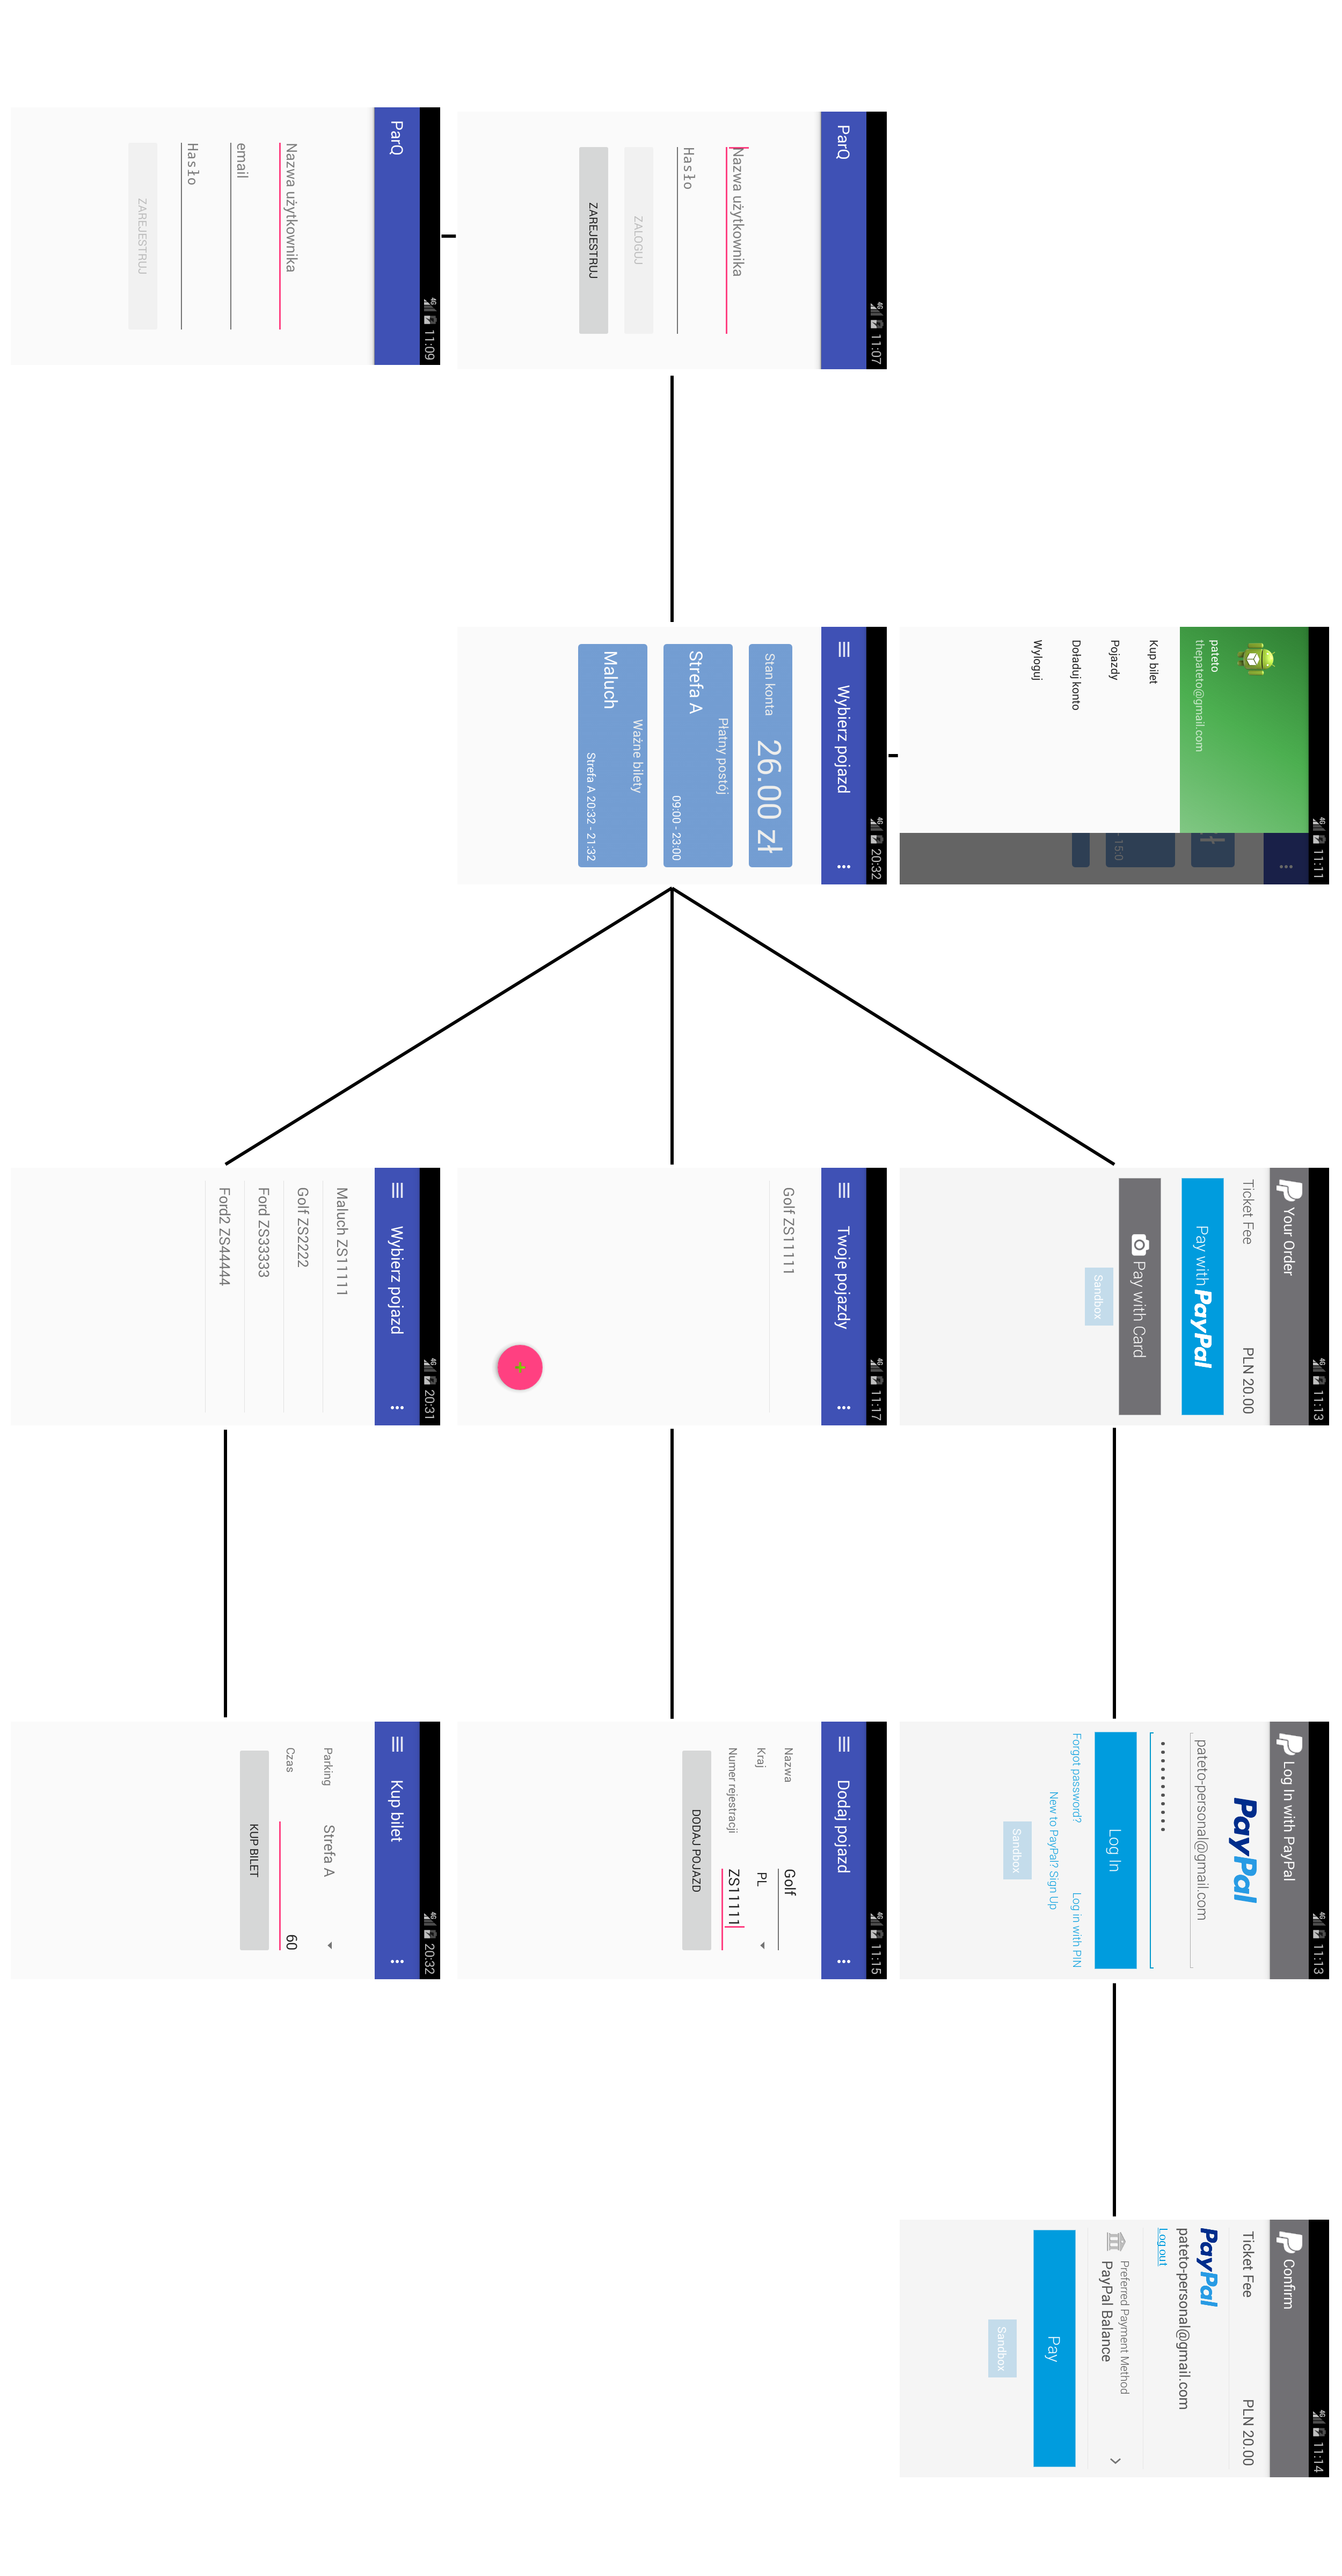
\includegraphics[width=0.7\linewidth]{05/all}
	\end{center}
	\caption{Ekrany w aplikacji kierowcy.}
	\label{przejscia_kierowca}
\end{figure}

\newpage

Druga z aplikacji umożliwiająca przeprowadzenie kontroli, a w jej skład wchodzą trzy ekrany. Po zalogowaniu, użytkownikowi prezentowany jest widok, na którym będą wyświetlane informacje o kontrolowanym pojeździe. Włączenie aparatu telefonu i rozpoczęcie przeprowadzania kontroli, zaczyna się w momencie dotknięcia przycisku ``Skanuj''. W chwili napotkania dowolnego kodu QR, skanowanie zostaje zakończone, a dane znajdujące się w kodzie są wysyłane do serwera systemu. Zwrócona odpowiedź jest prezentowana na ekranie, który był widoczny zaraz po zalogowaniu. To tutaj kontroler zostanie poinformowany o tym, czy kod jest poprawny i czy jest z nim powiązany obowiązujący bilet. W celu dalszej weryfikacji, prezentowana jest także informacja o numerze rejestracyjnym, aby można było sprawdzić czy plakietka z kodem QR jest powiązana z zaparkowanym pojazdem. Na rys. \ref{przejscia_kontroler} znajdują się ekrany aplikacji kontrolera.

\begin{figure}[h!]
	\begin{center}
		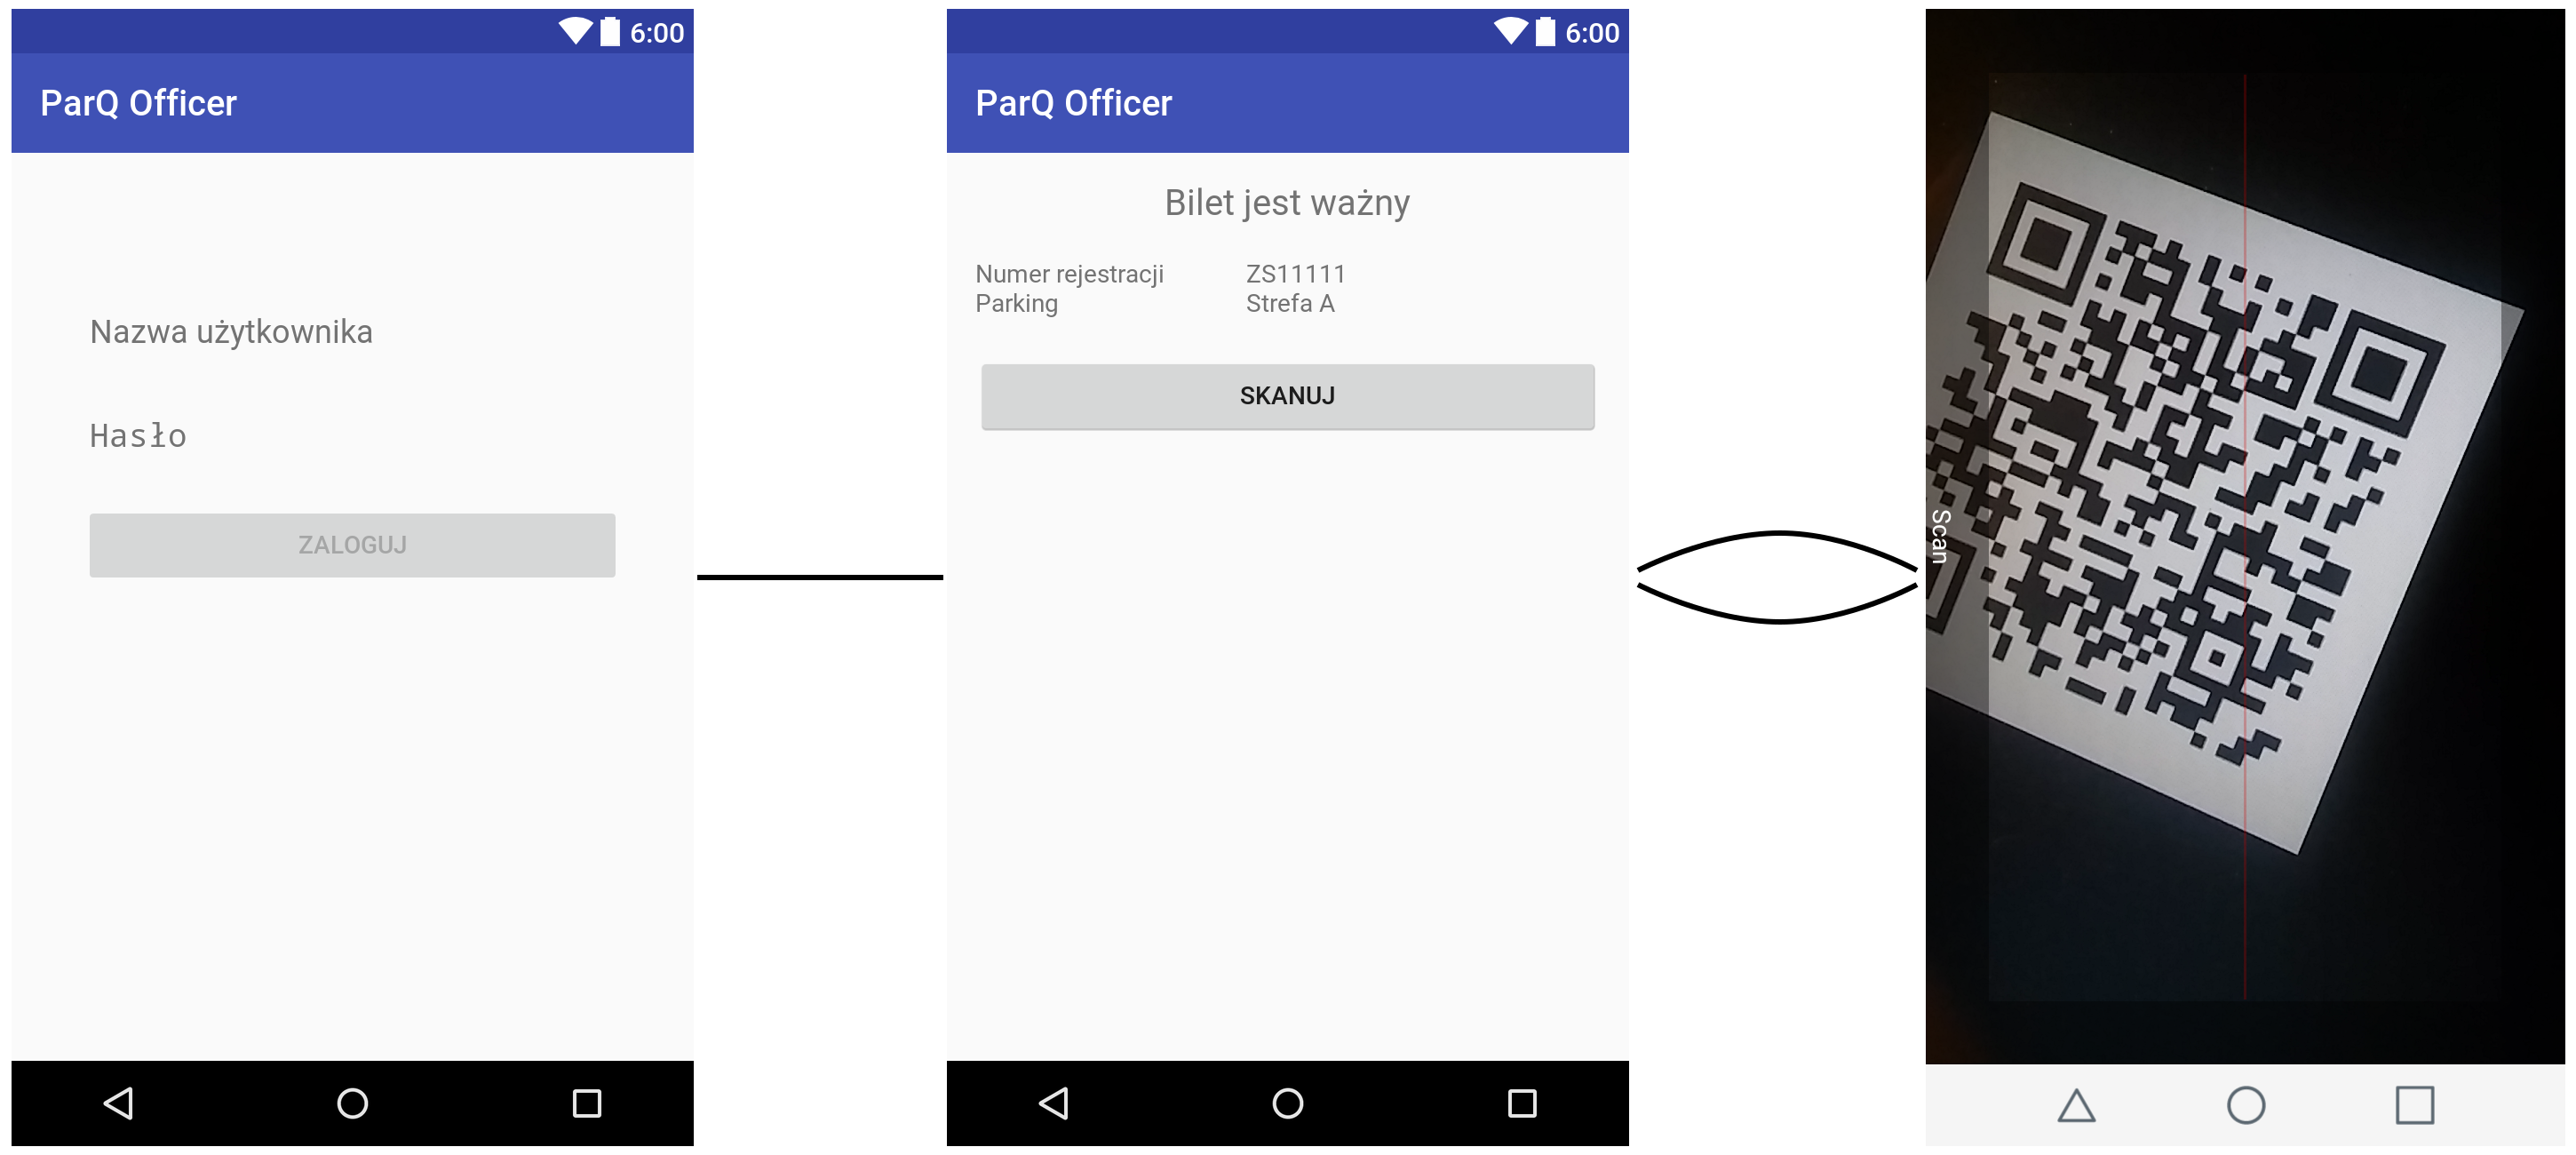
\includegraphics[width=0.7\linewidth]{05/all_officer}
	\end{center}
	\caption{Ekrany w aplikacji kontrolera.}
	\label{przejscia_kontroler}
\end{figure}

Cała funkcjonalność systemu dostępna z poziomu aplikacji mobilnych oparta jest na wymianie danych z serwerem. To właśnie udostępnianie odpowiedniego API jest głównym zadaniem aplikacji internetowej. W ten sposób tworzone są konta użytkowników, dodawane nowe pojazdy, kupowane oraz sprawdzane bilety. Oprócz tego system umożliwia także zarządzanie parkingiem, w tym dodawanie nowych grafików, taryfikatorów, czy tworzenie kont kontrolerów. To realizowane jest za pomocą strony administracyjnej, do której dostęp będą mieć pracownicy administracyjni. Strona ta została wygenerowana automatycznie przez framework Django, na bazie utworzonych modeli. Każdy z nich może być z jej poziomu tworzony, aktualizowany czy usuwany. Na rys. \ref{serwer_admin} została przedstawiona strona główna panelu administratora. Rys. \ref{serwer_schedule} przedstawia jedną z podstron, w której tworzony jest nowy grafik.

\newpage

\begin{figure}[p]
	\begin{center}
		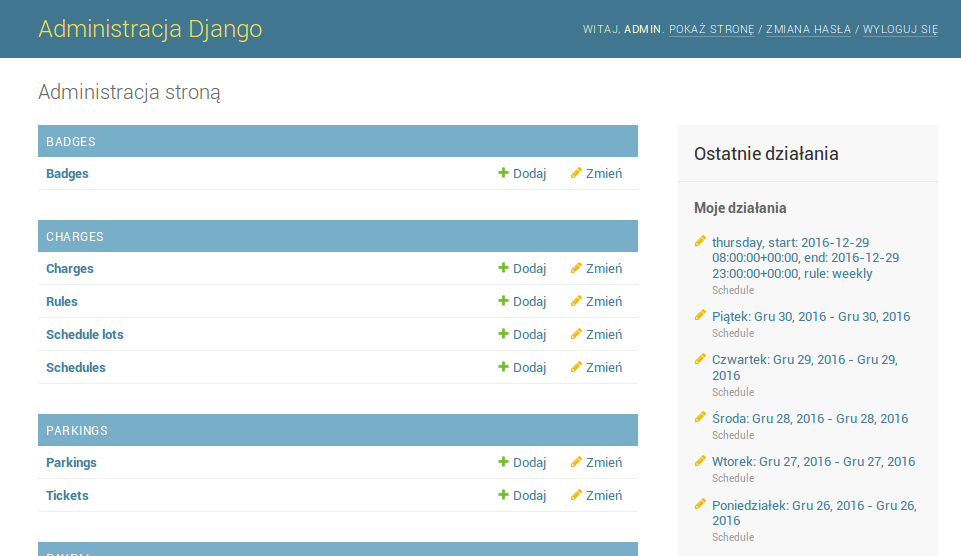
\includegraphics[width=0.9\linewidth]{05/admin_main}
	\end{center}
	\caption{Główny panel administratora.}
	\label{serwer_admin}
\end{figure}

\begin{figure}[p]
	\begin{center}
		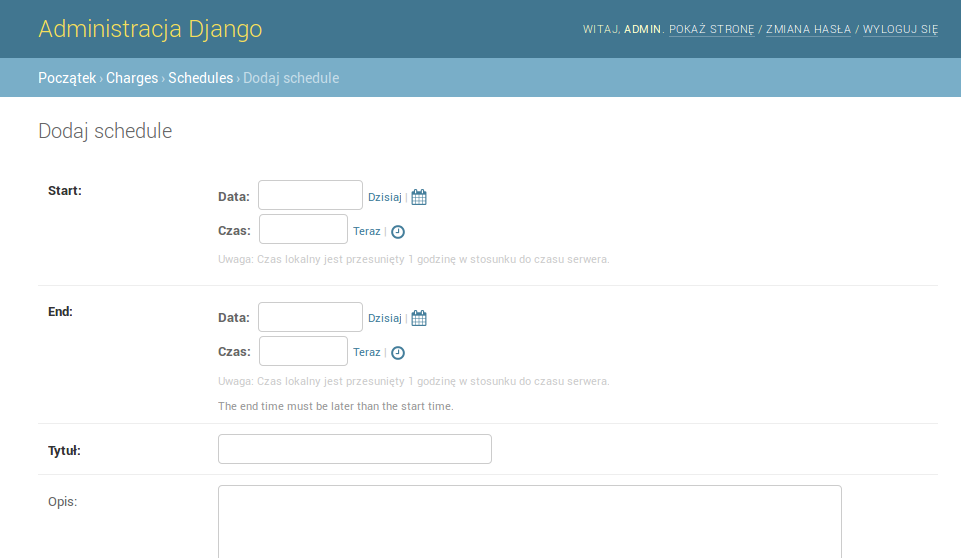
\includegraphics[width=0.9\linewidth]{05/admin_schedule}
	\end{center}
	\caption{Dodawanie nowego grafiku.}
	\label{serwer_schedule}
\end{figure}

\clearpage

\subsection{Testy}

Do weryfikowania poprawności tworzonego oprogramowania napisane zostały zestawy testów. Testy jednostkowe sprawdzają odpowiednie funkcjonowanie pojedynczych elementów systemu, takich jak metody klas. Poprawność interakcji zachodzących między modułami sprawdzana jest za pomocą testów integracyjnych. W aplikacji internetowej napisanej w Django, używana do tego celu jest klasa TestCase z pakietu django.test. Każdy z modułów tej aplikacji zawiera plik tests.py, w którym umieszczane są testy. Każdy z nich musi posiadać przynajmniej jedną asercję, która sprawdza poprawność otrzymanych danych i decyduje o sukcesie lub porażce przeprowadzonego testu. Podobnie sytuacja wygląda w Androidzie, gdzie używana jest biblioteka JUnit. Dodatkowo w celu dokładnego przetestowania, aplikacja mobilna była uruchamiana na emulatorze oraz rzeczywistym urządzeniu z systemem Android.
\\
\\
Akceptowanie transakcji przychodzących od klientów systemu wymaga posiadania specjalnego konta sprzedawcy. Dzięki PayPal Sandbox możliwe jest stworzenie środowiska testowego dla aplikacji, w którym mogą być utworzone fikcyjne konta klientów oraz sprzedawców. W ten sposób przeprowadzany jest cały proces płatności, który z perspektywy serwera i aplikacji mobilnej niczym nie różni się od prawdziwych transakcji. 

\subsection{Środowiska programistyczne i edytory}

Część mobilna systemu została wykonana w Android Studio, będącym dedykowanym środowiskiem programistycznym dla systemu Android. Zostało stworzone przez Google i bazuje na IntelliJ. Jest to rozbudowane IDE, które oprócz tworzenia gotowego szablonu aplikacji, posiada wszystkie funkcje spotykane w nowoczesnych środowiskach programistycznych, takie jak refaktoryzacja kodu, podpowiedzi, czy poprawianie składni. Razem z nim instalowany jest także emulator, dzięki czemu możliwe jest testowanie aplikacji bez potrzeby posiadania prawdziwego urządzenia z systemem Android.
\\
\\
Do pisania aplikacji serwerowej wykorzystywany był, dostępny z poziomu wiersza poleceń, edytor Vim. Jego standardowa funkcjonalność została rozszerzona o zewnętrzne dodatki, dzięki stworzonemu przez społeczność systemowi zarządzania rozszerzeniami -- Vundle. Do pracy wykorzystane zostały dodatki YouCompleteMe (okna z podpowiedziami i uzupełnianie kodu) i NERD Tree (wyświetlanie struktury plików).
		\newpage
		
		\section*{Podsumowanie}
\addcontentsline{toc}{section}{Podsumowanie}

Celem niniejszej pracy było stworzenie systemu płatności dla strefy płatnego parkowania. Do jego głównych zadań należało określenie wymagań systemu, zaimplementowanie serwera oraz aplikacji mobilnych. Użytkownicy korzystający z tego systemu mogą doładowywać swoje konta, rejestrować pojazdy oraz kupować bilety postojowe. Osoby kontrolujące mają możliwość sprawdzania ważności biletów postojowych. Główną cechą, która wyróżnia ten system spośród większości istniejących na rynku rozwiązań, jest zastosowanie kodów QR, za pomocą których identyfikowane są zaparkowane samochody. Postawiony w tej pracy cel został zrealizowany.
\\
\\
Pierwszy rozdział w większości poświęcony był płatnościom elektronicznym. W pierwszej części omówiona została Strefa Parkowania w Szczecinie oraz dokonano porównania systemu ParQ z już istniejącymi rozwiązaniami, które spełniają podobne zadania. Następnie dokonano analizy różnych metod płatności, pod kątem ich przydatności w systemach internetowych. Na bazie tych rozważań wybrana została forma zawierania transakcji, która najlepiej spełnia wymagania tworzonego systemu. W drugim rozdziale czytelnik został zapoznany z technologiami wykorzystywanymi do realizacji zadań pracy, a także pojęciami z nimi związanymi. Były one istotne dla pełnego zrozumienia dalszej części pracy. Kolejny rozdział zawiera dokumentację techniczną, natomiast ostatni, poświęcony został szczegółom implementacji.
\\
\\
Najbardziej pomocnymi pozycjami z bibliografii były publikacje o tematyce dotyczącej płatności elektronicznych. Szczególnie przydatna okazała się książka autorstwa Artura Borcucha, pt. \textit{Pieniądz elektroniczny pieniądz przyszłości -- analiza ekonomiczno-prawna}. W niezwykle wyczerpujący sposób opisane zostały w niej poszczególne etapy rozwoju pieniądza elektronicznego, które omówiono w rozdziale pierwszym. Szczególnie ważna na etapie implementacji systemu była dokumentacja Django, głównie dzięki przejrzystości oraz licznym przykładom w postaci fragmentów kodu, którymi opatrzone zostało prawie każde poruszane tam zagadnienie.
\\
\\
Mam nadzieję, że zebrane materiały okazały się wystarczające do zapoznania z zastosowanymi narzędziami oraz technologiami, użytymi do realizacji zadań pracy. Wybór tematu został podyktowany także rosnącą popularnością elektronicznych metod w internecie i aplikacjach mobilnych. Liczę, że podjęta analiza poruszonych tutaj zagadnień wykazała słuszność przyjętych rozwiązań. Praca nie wyczerpuje w pełni tematu, gdyż stworzony system ma szanse rozwoju w wielu kierunkach np.: wystawianie mandatu i rejestracja tego faktu na koncie użytkownika, powiadamianie kierowcy o zbliżającym się końcu opłaconego biletu.
		\newpage
		
		%\section*{Słownik pojęć}
\addcontentsline{toc}{section}{Słownik pojęć}

\begin{description}
	\item[E-commerce] -- (e-handel, ang. handel elektroniczny) blablabla bla blablbl a bla bll blla bldl, fds dsf  sjofds nosnfsd sjfosdj nkf.
	\item[Płatności elektroniczne] -- o płatnościach.
	\item[Dostawca usług płatniczych] -- PSP, MSP.
	\item[System płatniczy]
	\item[Instrument płatniczy]
	\item[Bankowość elektroniczna]
	\item[Bankowość internetowa]
	\item[Bankowość wirtualna]
\end{description}
		%\newpage
		\begin{raggedright}
			\bibliographystyle{plplain}
			\bibliography{bibfile.bib}
			\addcontentsline{toc}{section}{Literatura}
		\end{raggedright}
		\newpage
		
		\section*{Dodatek A. Spis zawartości dołączonej płyty CD}
\addcontentsline{toc}{section}{Dodatek A. Spis zawartości dołączonej płyty CD}

Na dołączonej płycie CD znajdują się:

\begin{itemize}
	\item praca\_inzynierska.pdf -- dokument z pracą inżynierską w formacie PDF,
	\item ParQ/driver\_app/ -- folder z aplikacją mobilną dla kierowcy,
	\item ParQ/officer\_app/ -- folder z aplikacją mobilną dla kontrolera,
	\item ParQ/server/ -- folder z projektem aplikacji internetowej,
	\item materialy/ -- folder z wybranymi materiałami wykorzystywanymi do realizacji pracy.
\end{itemize}

		\newpage
		
	\end{onehalfspacing}
\end{document}